\chapter{Mở đầu}
\label{ch:intro}

Chương này gồm bảy phần: (1) động lực của việc dùng mô hình ngôn ngữ nhỏ làm web agent; (2) phát biểu bài toán; (3) các thách thức; (4) mục tiêu và đóng góp; (5) phạm vi; (6) kết quả đạt được; và (7) bố cục của khóa luận.

\section{Bối cảnh và động lực}
\label{sec:intro-context}

Hãy hình dung một người quản lý cửa hàng trực tuyến, mỗi sáng đều lặp lại một chuỗi thao tác dường như không thay đổi trên trang quản trị: mở danh sách đơn hàng mới, kiểm tra đơn nào cần xử lý gấp, cập nhật trạng thái và trả lời những khách hàng đang chờ. Những thao tác này không đòi hỏi kiến thức chuyên môn hay khả năng suy luận phức tạp; phần lớn thông tin cần thiết đã được hiển thị trực tiếp trên giao diện. Thế nhưng, ngày qua ngày, con người vẫn phải tự mình thực hiện lại những công việc đó. Tình trạng tương tự xuất hiện trong vô số quy trình khác trên diễn đàn, trang tin tức, hệ thống quản trị hay các dịch vụ trực tuyến. Điểm chung của chúng là đều được thực hiện thông qua trình duyệt - một giao diện thống nhất để con người tiếp cận và điều khiển các dịch vụ web. Vì vậy, một agent có khả năng thao tác với website \emph{thông qua chính giao diện người dùng} có tiềm năng trở thành một dạng tự động hóa có phạm vi ứng dụng đặc biệt rộng.

Sự phát triển mạnh mẽ của các mô hình ngôn ngữ lớn (LLM) trong những năm gần đây đã tạo tiền đề để hiện thực hóa khả năng này. Thay vì phải lập trình cứng từng chuỗi thao tác, một web agent có thể nhận vào mục tiêu ở dạng ngôn ngữ tự nhiên, quan sát trạng thái của website, suy luận bước hành động tiếp theo và liên tục tương tác với giao diện cho đến khi hoàn thành nhiệm vụ. Cách tiếp cận này đã cho phép các agent thực hiện những chuỗi thao tác ngày càng phức tạp trên các môi trường web mô phỏng nhiều dịch vụ thực tế~\cite{sodhi2024step, yang2024agentoccam}.

Tuy nhiên, năng lực đó hiện vẫn phụ thuộc phần lớn vào các mô hình độc quyền có quy mô rất lớn và thường được cung cấp thông qua API. Sự phụ thuộc này tạo ra nhiều rào cản khi đưa web agent vào vận hành thực tế. Trước hết, một task thường bao gồm nhiều bước quan sát và tương tác, khiến chi phí tích lũy từ hàng loạt lần gọi API có thể trở nên đáng kể. Bên cạnh đó, độ trễ của máy chủ từ xa làm tăng thời gian hoàn thành task, đặc biệt đối với những quy trình dài. Đặc biệt hơn, việc gửi toàn bộ nội dung quan sát được từ website về máy chủ của bên thứ ba cũng đặt ra những lo ngại nghiêm trọng về quyền riêng tư, nhất là trong các hệ thống chứa dữ liệu nội bộ hoặc thông tin nhạy cảm. Cuối cùng, việc không kiểm soát được trọng số của mô hình khiến người triển khai khó có thể trực tiếp kiểm tra, điều chỉnh hoặc chuyên biệt hóa năng lực của agent cho một môi trường cụ thể.

Mô hình ngôn ngữ nhỏ (Small Language Model — SLM) vì thế trở thành một hướng tiếp cận hấp dẫn để giảm bớt những rào cản trên. Theo~\cite{belcak2025slm}, SLM chủ yếu được phân biệt bởi khả năng triển khai trên các thiết bị tiêu dùng phổ thông; trên thực tế, các mô hình có quy mô dưới mười tỷ tham số thường được xếp vào nhóm này. So với các LLM lớn, SLM có chi phí suy luận thấp hơn, có thể chạy cục bộ để hạn chế việc dữ liệu rời khỏi hệ thống, đồng thời cho phép người triển khai toàn quyền kiểm soát trọng số và thực hiện fine-tuning cho từng nhu cầu cụ thể.

Dẫu vậy, lợi thế về chi phí và khả năng triển khai đi kèm với một đánh đổi lớn về năng lực. Đây không phải là một bài toán dễ dàng ngay cả đối với những mô hình lớn nhất hiện nay. Trên WebArena - một benchmark gồm các bản sao website thực với đầy đủ chức năng và các task yêu cầu agent thực hiện nhiều bước tương tác — agent sử dụng GPT-4 chỉ hoàn thành khoảng 14\% số task tại thời điểm benchmark được công bố, trong khi con người đạt tới 78\%~\cite{zhou2024webarena}. Khoảng cách này cho thấy việc sử dụng trực tiếp một SLM chưa được chuyên biệt hóa khó có thể đáp ứng yêu cầu của các tác vụ web thực tế. Muốn thu hẹp khoảng cách đó, SLM cần được huấn luyện để học cách quan sát giao diện, lựa chọn hành động và phối hợp nhiều thao tác thành một chuỗi hoàn chỉnh.

Một hướng tiếp cận tự nhiên là fine-tuning có giám sát (Supervised Fine-Tuning — SFT) từ các trajectory thể hiện hành vi đúng của agent~\cite{lai2024autowebglm}. Tuy nhiên, cách tiếp cận này ngay lập tức đưa bài toán về một nút thắt khác: \textbf{dữ liệu huấn luyện}. Để một SLM có thể thực hiện tốt task trên một website cụ thể, cần có những trajectory mô tả chính xác cách hoàn thành các task trên website đó. Trong khi đó, các trajectory được gán nhãn mục tiêu trên từng website gần như không sẵn có ở quy mô lớn. Tự xây dựng chúng nhờ sức của con người lại đòi hỏi một lượng lớn thời gian và chi phí, đồng thời dữ liệu được tạo ra cho một website thường khó tái sử dụng trực tiếp cho website khác. Đây là một rào cản có tính hệ thống: khi mỗi website mới lại đòi hỏi một quy trình thu thập và gán nhãn dữ liệu gần như từ đầu, chi phí chuyên biệt hóa agent sẽ tăng theo số lượng môi trường cần hỗ trợ.

Chi phí này đã được thể hiện rõ trong các nghiên cứu trước. AutoWebGLM cần 20 người gán nhãn làm việc trong một tháng để xây dựng tập dữ liệu duyệt web của họ~\cite{lai2024autowebglm}. Ngược lại, Synatra cho thấy dữ liệu tổng hợp có thể giảm đáng kể chi phí tạo mẫu, với chi phí cho một mẫu tổng hợp chỉ khoảng 3\% so với một mẫu do con người tạo~\cite{ou2024synatra}. Những kết quả này gợi ý rằng thay vì tiếp tục mở rộng quy mô gán nhãn thủ công, một hướng đi khả thi hơn là \textbf{tự động hóa chính quá trình tạo dữ liệu huấn luyện}.

Đây chính là bài toán mà khóa luận này tập trung giải quyết. Mục tiêu là xây dựng một pipeline có khả năng tự động đi từ một website chưa được biết trước đến một tập dữ liệu có thể sử dụng để chuyên biệt hóa SLM. Pipeline thực hiện bốn bước chính: \emph{khám phá} website để tìm hiểu khả năng tương tác, \emph{tự tổng hợp} các task có ý nghĩa từ những gì đã khám phá, \emph{kiểm chứng} kết quả thực hiện và cuối cùng \emph{chuyển đổi} các trajectory hợp lệ thành dữ liệu huấn luyện. Với cách tiếp cận này, chi phí chuyên biệt hóa agent được chuyển từ một quy trình phụ thuộc nhiều vào nhân công sang một quy trình chủ yếu dựa trên chi phí tính toán, qua đó mở ra khả năng mở rộng sang nhiều website và nhiều môi trường khác nhau.

Tuy nhiên, tự động hóa việc khám phá không đơn giản là để agent tương tác ngẫu nhiên với website và ghi lại mọi trajectory thu được. Một chiến lược khám phá thiếu định hướng dễ dẫn đến việc lặp lại những thao tác quen thuộc, bỏ sót các chức năng quan trọng hoặc tạo ra những trajectory dài nhưng ít giá trị huấn luyện. Do đó, vấn đề cốt lõi của nghiên cứu không chỉ là \emph{khám phá được bao nhiêu}, mà còn là \emph{tích lũy và sử dụng tri thức đã khám phá như thế nào để tạo ra những task mới có giá trị}.

Từ đó, khóa luận đề xuất xây dựng một \emph{skill graph} để làm cấu trúc trung gian lưu trữ tri thức thu được trong quá trình khám phá. Mỗi skill đã được kiểm chứng được biểu diễn cùng với \emph{precondition} và \emph{effect} mà nó tạo ra trên trạng thái website. Thay vì xem mỗi trajectory là một chuỗi thao tác độc lập, hệ thống có thể xem chúng như những thành phần có thể tái sử dụng. Các skill trong đồ thị sau đó được \emph{ghép nối} dựa trên quan hệ giữa precondition và effect để hình thành những task dài hơn, đa dạng hơn và có ngữ nghĩa hoàn chỉnh.

Theo hướng tiếp cận này, quá trình tạo dữ liệu không còn là việc đơn thuần thu thập thật nhiều trajectory, mà trở thành một quá trình \textbf{khám phá, tích lũy, kiểm chứng và tái tổ hợp tri thức}. Đây là nền tảng để xây dựng một pipeline có khả năng tự động tạo ra dữ liệu huấn luyện chất lượng cao, qua đó giảm sự phụ thuộc vào gán nhãn thủ công và hỗ trợ việc chuyên biệt hóa SLM cho các môi trường web khác nhau với chi phí thấp hơn.

\section{Phát biểu bài toán}
\label{sec:intro-problem}

Bài toán của khóa luận được phát biểu như sau.

\begin{quote}
  \textbf{Cho} (i) một website đang hoạt động,
  truy cập được qua trình duyệt tiêu chuẩn, và (ii) một mô hình ngôn ngữ nhỏ đã
  được huấn luyện, \textbf{hãy tạo ra} phiên bản fine-tune của mô hình đó để nó có khả
  năng hoàn thành các task phát biểu bằng ngôn ngữ tự nhiên trên website,
  \textbf{mà không dùng} đến3 dữ liệu huấn luyện có sẵn hoặc do con người tạo.
\end{quote}

Giao diện tương tác của agent được tuân
theo các thiết lập tiêu chuẩn của bài toán web agent. Cụ thể, ở mỗi bước,
mô hình sẽ phân tích trạng thái môi trường thông qua URL hiện tại và
accessibility tree - bản mô tả cấu trúc văn bản của giao diện người dùng
đang hiển thị. Tiếp đó, hệ thống sẽ quyết định và thực thi một hành động thuộc
action space đã được định nghĩa từ trước, bao gồm: nhấp chuột,
nhập văn bản, chọn menu, điều hướng, hoặc báo cáo trạng thái task (đã hoàn thành
hoặc bất khả thi). Khi đó, một \emph{trajectory} chính là chuỗi tuần tự các cặp
(quan sát, hành động) được sinh ra trong suốt quá trình agent thực hiện một mục tiêu cụ thể.

Điểm mấu chốt nằm ở việc xây dựng tập dữ liệu huấn luyện. Quá trình fine-tuning cần một tập dữ liệu
$D = \{(g_i, \tau_i)\}$ gồm các mục tiêu kèm trajectory thành công. Vì vậy
câu hỏi thực chất là câu hỏi \emph{sinh dữ liệu}: làm thế nào để tự động tạo ra
các mục tiêu $g_i$ có ý nghĩa trên website này và thu thập các trajectory
$\tau_i$ tương ứng, đồng thời bảo đảm rằng chúng thực sự hoàn thành các mục tiêu đó (có thể kiểm chứng được)?
Chất lượng của phương pháp được đánh giá thông qua mục tiêu cuối cùng: mô hình sau fine-tune được đánh giá theo
\emph{tỷ lệ hoàn thành task} trên bộ task chính thức, chấm điểm tự động,
của benchmark WebArena~\cite{zhou2024webarena}, so với chính mô hình đó
trước khi fine-tune.

\section{Thách thức}
\label{sec:intro-challenges}

Quá trình tự động hóa việc thu thập dữ liệu và huấn luyện web agent phải đối mặt với năm thách thức kỹ thuật cốt lõi:

\begin{enumerate}
  \item \textbf{Khó khăn trong việc thu thập dữ liệu chất lượng cao.} Việc huấn luyện web agent đòi hỏi tập dữ liệu trajectory tương tác với giao diện (GUI) với quy mô lớn và độ chính xác cao. Dữ liệu do con người trực tiếp thao tác và gán nhãn có thể đảm bảo tính chuẩn xác nhưng đòi hỏi chi phí nhân lực và thời gian rất lớn, không thể mở rộng quy mô một cách bền vững. Ngược lại, các phương pháp tự động sinh dữ liệu từ tri thức gián tiếp hoặc tài liệu hướng dẫn tĩnh trên Internet không phản ánh được tính động và các ràng buộc trạng thái thực tế của môi trường web, dẫn đến hiệu năng hạn chế khi triển khai.
  \item \textbf{Thiếu hiểu biết trước về môi trường triển khai.} Các web agent thường không có tri thức về cấu trúc, sơ đồ điều hướng và luồng chức năng của website cần thực hiện tác vụ. Khi hoạt động trên các website lạ, agent gặp khó khăn trong việc xác định các trang cần duyệt để đạt trạng thái đích. Các phương pháp khám phá không có cấu trúc dễ bị rơi vào trạng thái lặp lại thao tác tại các trang dễ tiếp cận, đồng thời bỏ sót các chức năng nằm sâu trong cấu trúc phân cấp của website.
  \item \textbf{Khả năng chuyển giao (transfer) kém.} Tri thức tương tác và các trajectory thu thập từ một website cụ thể có tính đặc thù cao theo cấu trúc DOM và luồng nghiệp vụ riêng của website đó, khiến khả năng chuyển giao sang các môi trường web khác bị suy giảm rõ rệt. Do sự khác biệt lớn về phân phối giao diện giữa các ứng dụng, mô hình cần được học và thích ứng trực tiếp từ chính môi trường mà agent sẽ vận hành thực tế.
  \item \textbf{Kiểm chứng tính đúng đắn.} Trong quy trình tự sinh dữ liệu không có sự giám sát của con người, agent tự đề xuất task và tự thực thi hành động. Nếu hệ thống ghi nhận thành công chỉ dựa trên phán đoán tự thân của agent, tập dữ liệu sẽ chứa nhiều trajectory không đạt yêu cầu (chẳng hạn như việc agent tuyên bố hoàn thành task mà không tạo ra bất kỳ tác động nào lên trạng thái của trang). Việc đưa các mẫu dữ liệu này vào huấn luyện sẽ dạy mô hình thói quen báo hoàn thành sớm hoặc bỏ cuộc.
  \item \textbf{Ghép các task ngắn thành semantic task.} Các cơ chế đề xuất task dựa trên trạng thái của một trang đơn lẻ chỉ tạo ra các task cục bộ với phạm vi ngắn hạn (từ một đến hai bước thao tác). Trong khi đó, các yêu cầu thực tế của người dùng thường là những semantic task nhiều bước, đòi hỏi sự phối hợp tuần tự giữa nhiều skill qua các trạng thái trang khác nhau. Việc xây dựng các task dài hạn có ý nghĩa đòi hỏi phải mô hình hóa được quan hệ phụ thuộc tiền điều kiện (precondition) và hiệu ứng (effect) giữa các skill độc lập, vốn là thông tin không thể suy luận từ một trang riêng lẻ.
\end{enumerate}

\section{Mục tiêu và đóng góp}
\label{sec:intro-contrib}

Khóa luận theo đuổi năm mục tiêu:

\begin{enumerate}
  \item[\textbf{O1.}] \textbf{Khám phá tự động:} Xây dựng cơ chế khám phá có cấu trúc dựa trên đồ thị nhằm tự động thu thập các trajectory tương tác từ các website thực tế mà không cần dữ liệu mẫu hay tri thức từ con người.
  \item[\textbf{O2.}] \textbf{Sinh semantic task:} Phát triển phương pháp tự động phát hiện và trừu tượng hóa các skill có thể tái sử dụng thành các planning operator, từ đó ghép chuỗi chúng trên đồ thị để tạo ra các semantic task có ý nghĩa nghiệp vụ trên website đang khám phá.
  \item[\textbf{O3.}] \textbf{Kiểm chứng và tinh lọc dữ liệu:} Thiết lập quy trình tinh lọc dữ liệu tự động với các chốt chặn kiểm tra tính đúng đắn đa tầng, đồng thời đảm bảo tính nhất quán giữa dữ liệu huấn luyện và suy luận theo nguyên tắc \emph{prompt parity}.
  \item[\textbf{O4.}] \textbf{Fine-tuning và đánh giá mô hình:} Fine-tune mô hình ngôn ngữ nhỏ (SLM) trên tập dữ liệu tương tác đã sinh từ luồng khám phá và đánh giá năng lực giải quyết task của mô hình đó trên bộ chuẩn WebArena.
  \item[\textbf{O5.}] \textbf{Tổng kết kinh nghiệm thực tiễn:} Phân tích những hạn chế thực tế (đặc biệt ở execution layer) và đúc kết các bài học kỹ thuật thành bộ hướng dẫn thực hành tốt (best practices) khi xây dựng web agent.
\end{enumerate}

Bảng~\ref{tab:contrib} phân định rõ ranh giới giữa những tài nguyên khóa luận kế thừa và những đóng góp mới. Nhìn chung, khóa luận mang lại năm đóng góp cốt lõi. Đầu tiên là phương pháp HSGE: một chu trình khám phá và ghép chuỗi dựa trên đồ thị với kiến trúc task hai tầng. Trong kiến trúc đó, các low-level task do LLM đề xuất dẫn dắt quá trình khám phá, còn các semantic task sinh ra từ operator graph cung cấp dữ liệu dài hạn. Thứ hai là bộ tinh lọc dữ liệu tự động, gồm các cổng chất lượng chấm lại từng episode ngay trong vòng lặp thu thập, được tích hợp vào một trình dựng dữ liệu tuân thủ nguyên tắc prompt parity. Ba đóng góp còn lại là: một mô hình web agent 9B đã fine-tune cùng tập dữ liệu đã thu; kết quả đánh giá mô hình đó trên bộ task WebArena chính thức; và một báo cáo kinh nghiệm vận hành các chu trình tương tự.

\begin{table}[htbp]
  \centering
  \caption[Tài nguyên kế thừa và đóng góp của khóa luận]{Phân định tài nguyên kế thừa và các đóng góp cốt lõi của khóa luận.}
  \label{tab:contrib}
  \small
  \begin{tabular}{@{}L{6.4cm} L{6.8cm}@{}}
    \toprule
    \textbf{Tài nguyên có sẵn (sử dụng nguyên bản)} & \textbf{Đóng góp của khóa luận} \\
    \midrule
    Các website, task và hệ thống đánh giá của WebArena~\cite{zhou2024webarena};
    giao diện trình duyệt BrowserGym~\cite{dechezelles2025browsergym} &
    Chu trình HSGE: đồ thị hai tầng, khám phá có định hướng, phát hiện và kiểm
    chứng skill (Chương~\ref{ch:method}) \\
    \addlinespace
    Mô hình gốc Qwen3.5-9B~\cite{qwen2026qwen35}; LoRA~\cite{hu2022lora};
    LLaMA-Factory~\cite{zheng2024llamafactory}; vLLM~\cite{kwon2023vllm} &
    Sinh semantic task bằng cách ghép chuỗi operator, kết hợp cơ chế induction nhận thức từ vựng và cổng chặn tautology (Mục~\ref{sec:method-semantic}) \\
    \addlinespace
    Bộ mã hóa sentence embedding~\cite{reimers2019sbert};
    khung hình thức options, STRIPS và các công trình nâng options thành operator
    ký hiệu~\cite{sutton1999options,fikes1971strips,konidaris2009skillchaining,konidaris2018skills2symbols} &
    Tinh lọc dữ liệu tự động (LLM judge, cấu trúc lại suy luận) và trình dựng dataset
    prompt-parity (Mục~\ref{sec:method-data}); tập dữ liệu và mô hình
    fine-tune (Chương~\ref{ch:experiments}); báo cáo kinh nghiệm kỹ thuật
    (Mục~\ref{sec:disc-lessons}, Phụ lục~\ref{app:lessons}) \\
    \bottomrule
  \end{tabular}
\end{table}
\section{Câu hỏi nghiên cứu}
\label{sec:intro-rq}

Năm mục tiêu nghiên cứu trên được cụ thể hóa thành bốn câu hỏi nghiên cứu (Research Questions). Toàn bộ thiết kế thực nghiệm và phân tích ở Chương~\ref{ch:experiments} và Chương~\ref{ch:discussion} được xây dựng nhằm trả lời các câu hỏi này:

\begin{enumerate}
  \item[\textbf{CH1.}] \textbf{Hiệu quả thu thập dữ liệu và chi phí khám phá:} Pipeline khám phá tự động thu thập được bao nhiêu dữ liệu và tri thức có cấu trúc (skill, operator, semantic task) khi vận hành trên các website thực tế, tỷ lệ dữ liệu hợp lệ vượt qua các cổng kiểm soát chất lượng là bao nhiêu, và mức chi phí API/tài nguyên tính toán trên mỗi trajectory đạt được lợi thế kinh tế như thế nào?
  \item[\textbf{CH2.}] \textbf{Mức độ cải thiện năng lực của mô hình ngôn ngữ nhỏ:} Việc fine-tune trên tập dữ liệu tương tác tự sinh nâng cao hiệu năng của mô hình ngôn ngữ nhỏ (SLM) ở mức độ nào trên các website mục tiêu, và sự cải thiện này chủ yếu đến từ năng lực suy luận hành động hay khả năng tuân thủ định dạng tương tác?
  \item[\textbf{CH3.}] \textbf{So sánh tương quan về hiệu năng và chi phí với các giải pháp hiện hành:} Hiệu năng của mô hình sau fine-tune định vị ở đâu so với các hệ thống mã nguồn mở dưới 10 tỷ tham số hiện nay trên bộ chuẩn WebArena, và pipeline HSGE đạt được lợi thế gì về mặt chi phí thu thập dữ liệu (với chi phí API chỉ khoảng 0{,}0358\,USD mỗi trajectory) khi so sánh với các công trình cùng hướng tiếp cận như Go-Browse?
  \item[\textbf{CH4.}] \textbf{Phân tích nguyên nhân thất bại và điểm nghẽn hệ thống:} Những yếu tố nào chi phối chủ yếu đến các ca thất bại của agent, và đâu là các rào cản kỹ thuật cốt lõi (đặc biệt ở execution layer và cơ chế phục hồi lỗi) ảnh hưởng trực tiếp đến tỷ lệ hoàn thành task của web agent?
\end{enumerate}

Bảng~\ref{tab:rqmap} chỉ ra nơi mỗi câu hỏi nghiên cứu được đo lường thực nghiệm và nơi được phân tích trả lời chi tiết.

\begin{table}[htbp]
  \centering
  \caption[Bảng ánh xạ câu hỏi nghiên cứu]{Ánh xạ giữa bốn câu hỏi nghiên
  cứu, mục tiêu tương ứng, số liệu dùng để trả lời và mục trả lời.}
  \label{tab:rqmap}
  \small
  \begin{tabular}{@{}l L{3.5cm} L{4.3cm} L{2.7cm}@{}}
    \toprule
    \textbf{Câu hỏi} & \textbf{Mục tiêu} & \textbf{Số liệu dùng để trả lời} &
    \textbf{Trả lời ở} \\
    \midrule
    CH1 & O1, O2 &
    Mục~\ref{sec:exp-data}, \ref{sec:exp-cost-explore} (Bảng~\ref{tab:runs}, \ref{tab:dataset}, \ref{tab:apicost}) &
    Mục~\ref{sec:disc-results} \\
    \addlinespace
    CH2 & O3, O4 &
    Mục~\ref{sec:exp-main}, \ref{sec:exp-baseline}
    (Bảng~\ref{tab:baseline}, \ref{tab:profile}) &
    Mục~\ref{sec:disc-results} \\
    \addlinespace
    CH3 & O4 &
    Mục~\ref{sec:exp-main}, \ref{sec:exp-cost-explore} (Bảng~\ref{tab:related}, \ref{tab:apicost}) &
    Mục~\ref{sec:disc-results}, \ref{sec:disc-related} \\
    \addlinespace
    CH4 & O1--O5 &
    Mục~\ref{sec:exp-analysis} (Bảng~\ref{tab:crosssite}, \ref{tab:failures}) &
    Mục~\ref{sec:disc-results} \\
    \bottomrule
  \end{tabular}
\end{table}

\section{Phạm vi}
\label{sec:intro-scope}

Để đảm bảo tính tập trung và khả năng kiểm soát thực nghiệm, khóa luận xác định phạm vi nghiên cứu theo bốn khía cạnh sau:

\begin{enumerate}
  \item \textbf{Môi trường thực nghiệm và benchmark:} Nghiên cứu được tiến hành trên bốn website được nhóm tự triển khai (self-hosted) thuộc benchmark WebArena~\cite{zhou2024webarena} bao gồm: \emph{Shopping (Magento), Shopping Admin, GitLab} và \emph{Reddit (Postmill)}, với tổng cộng 655 task dùng để đánh giá mô hình và có bộ chấm tự động. Nghiên cứu loại trừ website \emph{Map} do đặc thù tương tác bản đồ đòi hỏi phải xử lý về mặt thị giác. Agent vận hành dựa trên các phiên đăng nhập chuẩn đã được cấu hình sẵn; việc giải CAPTCHA, vượt cơ chế chống bot hay tương tác với các dịch vụ web công cộng bên ngoài nằm ngoài phạm vi đề tài.
  \item \textbf{Không gian quan sát và hành động:} Agent sử dụng không gian quan sát dựa trên cây tiếp cận (Accessibility Tree) đã làm phẳng của BrowserGym~\cite{dechezelles2025browsergym}, kết hợp với URL và lịch sử thao tác; không sử dụng ảnh chụp màn hình (screenshot) làm đầu vào cho mô hình ngôn ngữ trong quá trình fine-tuning và suy luận. Không gian hành động tuân thủ theo tiêu chuẩn của trình duyệt (\texttt{click}, \texttt{fill}, \texttt{press\_key}, \texttt{go\_back}, \dots).
  \item \textbf{Mô hình và phương pháp huấn luyện:} Khóa luận tập trung vào phương pháp tinh chỉnh tham số hiệu quả (LoRA SFT) trên mô hình ngôn ngữ nhỏ (SLM) mã nguồn mở phân khúc dưới 10 tỷ tham số (cụ thể là Qwen3.5-9B), với ngôn ngữ là tiếng Anh. Các kỹ thuật học tăng cường (RL), tối ưu theo sở thích (DPO/PPO/GRPO) hay huấn luyện mô hình đa phương thái (VLM) không thuộc phạm vi nghiên cứu này.
  \item \textbf{Ranh giới thực nghiệm:} Xuất phát từ giới hạn về ngân sách nghiên cứu và tài nguyên tính toán trong phạm vi một khóa luận ở bậc đại học, đề tài ưu tiên hoàn thành trọn vẹn chu trình thực nghiệm từ đầu đến cuối (HSGE) và đánh giá sự cải thiện năng lực của mô hình SLM sau fine-tune trên benchmark WebArena. Việc thực hiện các thực nghiệm ablation cô lập biến số quy mô lớn trên từng module độc lập (đòi hỏi lặp lại toàn bộ quá trình thu thập và nhân bội ngân sách API/GPU) nằm ngoài phạm vi khả thi của đề tài và được định hướng như công việc tương lai.
\end{enumerate}

\section{Kết quả đạt được}
\label{sec:intro-results}

Quá trình triển khai thực nghiệm agent HSGE trên bốn website thuộc benchmark WebArena đã mang lại các kết quả định lượng và phát hiện khoa học cốt lõi sau:

\textbf{1. Khối lượng dữ liệu và tri thức tự động thu thập:}
Pipeline khám phá đã duyệt qua 455 trang web (node), ghi nhận 3981 episode tương tác, từ đó phát hiện 146 skill có thể tái sử dụng và quy nạp thành công 57 operator (Bảng~\ref{tab:runs}). Trên cơ sở đó, hệ thống tự động sinh và giải 142 semantic task nhiều bước. Sau khi đi qua các cổng kiểm soát chất lượng tự động, 1760 trajectory hợp lệ được chuyển đổi thành 9007 mẫu dữ liệu (gồm 8554 mẫu train và 453 mẫu validation) mà không cần đến bất kỳ sự can thiệp hay gán nhãn thủ công nào từ con người (Bảng~\ref{tab:dataset}).

\textbf{2. Cải thiện hiệu năng của mô hình ngôn ngữ nhỏ (Phát hiện 1):}
Mô hình Qwen3.5-9B sau khi fine-tune bằng LoRA trên tập dữ liệu tự sinh đạt tỷ lệ hoàn thành tác vụ \textbf{24,6\%} trên toàn bộ 655 task chính thức của bốn website, tăng \textbf{+11,3 điểm phần trăm} so với mô hình gốc chưa fine-tune (13,3\%). Mức cải thiện này đạt ý nghĩa thống kê trên cả bốn website theo kiểm định McNemar theo cặp ($p < 0{,}001$, Bảng~\ref{tab:baseline}). Khi đối sánh với các mô hình cùng phân khúc dưới 10 tỷ tham số, kết quả này vượt qua NNetNav-7B (19,1\%), GPT-4o-mini (20,0\%) và đạt mức tương đương với Go-Browse-7B (22,6\%) (Bảng~\ref{tab:related}).

\textbf{3. Cải thiện đồng thời cả tính chuẩn xác về cú pháp lệnh lẫn năng lực suy luận chọn hành động (Phát hiện 2):}
Phân tích chi tiết chân dung lỗi cho thấy sự cải thiện hiệu năng của mô hình đến từ hai khía cạnh rõ rệt:
\begin{itemize}
  \item \emph{Khả năng tuân thủ định dạng và cú pháp hành động:} Mô hình học được cách xuất ra câu lệnh Python hợp lệ mà trình duyệt có thể thực thi được, giảm tỷ lệ phiên bị hủy do lỗi cú pháp từ 26,0\% ở mô hình gốc xuống chỉ còn 0,6\% sau khi fine-tune (đóng góp trực tiếp vào 47 task giải được thêm).
  \item \emph{Năng lực suy luận và lựa chọn hành động:} Trên tập 485 task mà mô hình gốc vốn đã xuất đúng cú pháp, tỷ lệ giải thành công của mô hình sau fine-tune vẫn tăng từ 17,9\% lên 23,5\% với ý nghĩa thống kê ($p = 0{,}003$). Điều này chứng minh dữ liệu huấn luyện thực sự giúp mô hình nâng cao năng lực ra quyết định trên trang web, chứ không chỉ đơn thuần là học cách bắt chước khuôn mẫu cú pháp bên ngoài.
\end{itemize}

\textbf{4. Rào cản cốt lõi nằm ở tầng thực thi thay vì quy mô dữ liệu (Phát hiện 3):}
Thống kê thất bại chỉ ra rằng từ 85\% đến 96\% số episode không hoàn thành có ít nhất một hành động bị trình duyệt từ chối (chủ yếu do lỗi timeout khi tương tác với các phần tử DOM phức tạp) (Bảng~\ref{tab:failures}). Ngoài ra, website có lượng dữ liệu huấn luyện lớn nhất (Shopping Admin, chiếm 41,9\%) lại chỉ xếp thứ ba về tỷ lệ thành công (Bảng~\ref{tab:crosssite}). Điều này cho thấy việc tiếp tục tăng khối lượng dữ liệu thuần túy sẽ mang lại hiệu quả biên giảm dần; hướng đầu tư quan trọng tiếp theo là nâng cao độ tin cậy của tầng thực thi (execution layer) và trang bị cơ chế tự phục hồi sau lỗi thao tác.

\textbf{5. Hiệu quả kinh tế và tính khả thi trong điều kiện tài nguyên giới hạn:}
Toàn bộ giai đoạn khám phá và thu thập dữ liệu được thực hiện với chi phí gọi API là \textbf{36,48 USD} (trung bình khoảng \textbf{0,0358 USD} cho mỗi trajectory thành công đưa vào tập huấn luyện, Bảng~\ref{tab:apicost}). So với mức chi phí API $\approx 0{,}0976$ USD/trajectory của Go-Browse~\cite{gandhi2026gobrowse} (tổng cộng 975,57 USD), chu trình HSGE có chi phí thu thập rẻ hơn \textbf{gần 2,7 lần} trên mỗi mẫu dữ liệu thành công, đồng thời tiết kiệm hàng trăm lần so với quy trình gán nhãn thủ công tiêu tốn hàng nghìn USD~\cite{lai2024autowebglm}. Kết quả này chứng minh tính khả thi kinh tế vượt trội của phương pháp, mở ra cơ hội tiếp cận cho các nhóm nghiên cứu có nguồn lực tài chính hạn chế ở quy mô luận văn.

\textbf{6. Sản phẩm bàn giao và giới hạn nghiên cứu:}
Đề tài bàn giao bốn hiện vật hoàn chỉnh gồm: mã nguồn của agent HSGE; bộ dữ liệu 9007 mẫu; checkpoint mô hình đã fine-tune; và báo cáo kinh nghiệm vận hành thực tế (Phụ lục~\ref{app:lessons}). Do giới hạn tài nguyên của một khóa luận đại học, các kết quả đối chứng được thu thập từ một lượt chạy chuẩn hóa trên 655 task của benchmark; các thực nghiệm ablation lặp lại nhiều lần được đề xuất cho các nghiên cứu tiếp theo.

\section{Bố cục khóa luận}
\label{sec:intro-organization}

Chương 1 tóm tắt lộ trình nghiên cứu và vị trí của từng
chương trên lộ trình đó. Chương~\ref{ch:related} trình bày kiến thức nền và
định vị khóa luận giữa các công trình liên quan. Chương~\ref{ch:method}
trình bày trọn vẹn pipeline HSGE, từ khám phá đến mô hình đã fine-tune.
Chương~\ref{ch:experiments} đánh giá pipeline: dữ liệu nó thu thập, mô hình
nó tạo ra, và hiệu năng của mô hình đó trên benchmark chính thức.
Chương~\ref{ch:discussion} trả lời lần lượt các câu hỏi nghiên cứu và tóm
tắt các bài học kỹ thuật, phần đầy đủ nằm ở Phụ lục~\ref{app:lessons}. Chương~\ref{ch:conclusion} kết luận và nêu hướng phát triển.
Hình~\ref{fig:bigpicture} tóm tắt lộ trình đó và vị trí của từng chương
trên lộ trình.

\begin{figure}[H]
  \centering
  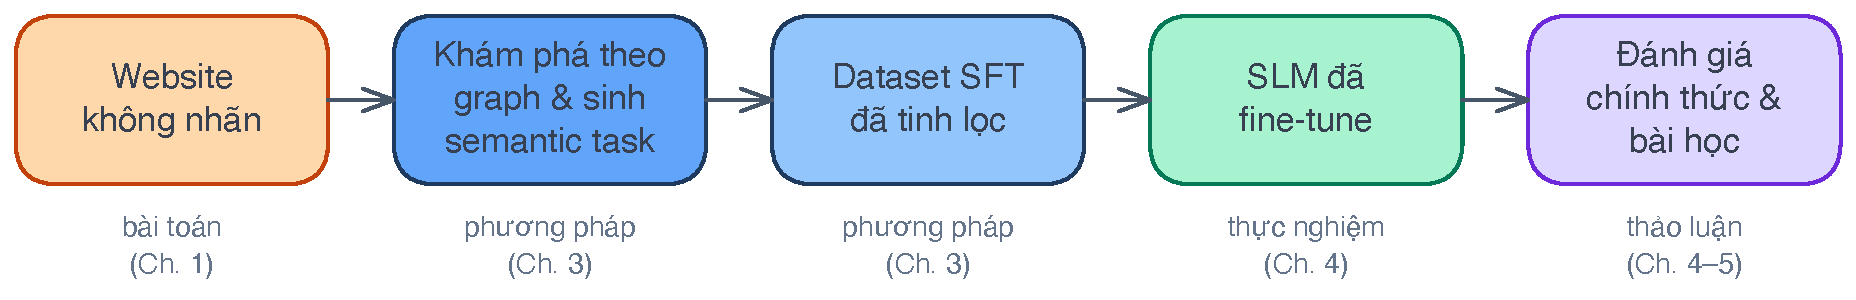
\includegraphics[width=\textwidth]{Figures/fig_roadmap.pdf}
  \caption[Lộ trình nghiên cứu của khóa luận]{Lộ trình nghiên cứu: từ một
    website không nhãn đến một mô hình ngôn ngữ nhỏ được đánh giá chính thức,
  cùng các chương phụ trách từng giai đoạn.}
  \label{fig:bigpicture}
\end{figure}

\vspace{0.5em}
\noindent
Ở chương~2, chúng tôi sẽ đặt lộ trình này vào bức tranh các nghiên cứu hiện có.
